\documentclass[12pt]{article}
\usepackage[utf8]{inputenc}
\usepackage{subfigure}
\usepackage{graphicx}
%\graphicspath{{images/}}
\usepackage[left=0cm,top=1cm,right=0cm,bottom=0.2cm]{geometry}
\begin{document}

\begin{figure}[h!]
\centering
  \begin{subfigure}
      \centering
    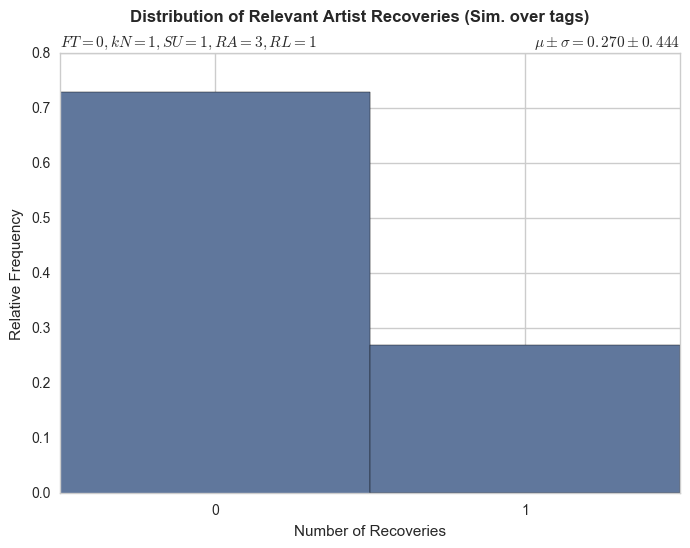
\includegraphics[height=2.4in]{tags,FT=0,kN=1,SU=1,RA=3,RL=1.png}
  \end{subfigure}
  \begin{subfigure}
      \centering
    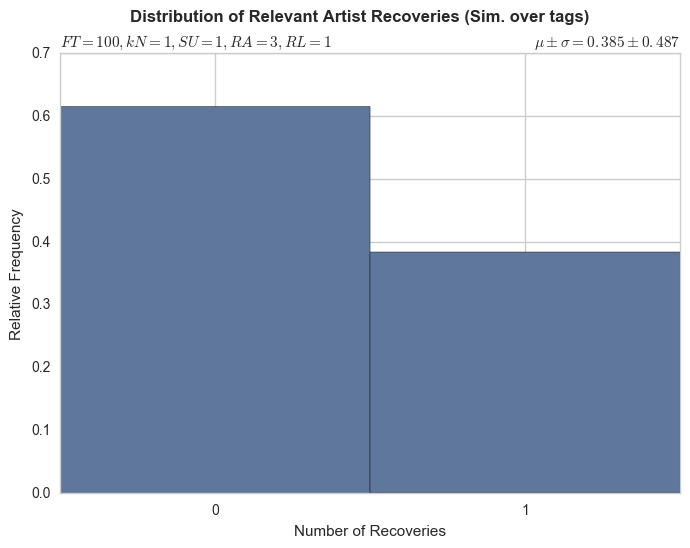
\includegraphics[height=2.4in]{tags,FT=100,kN=1,SU=1,RA=3,RL=1.png}
  \end{subfigure}
  \begin{subfigure}
      \centering
    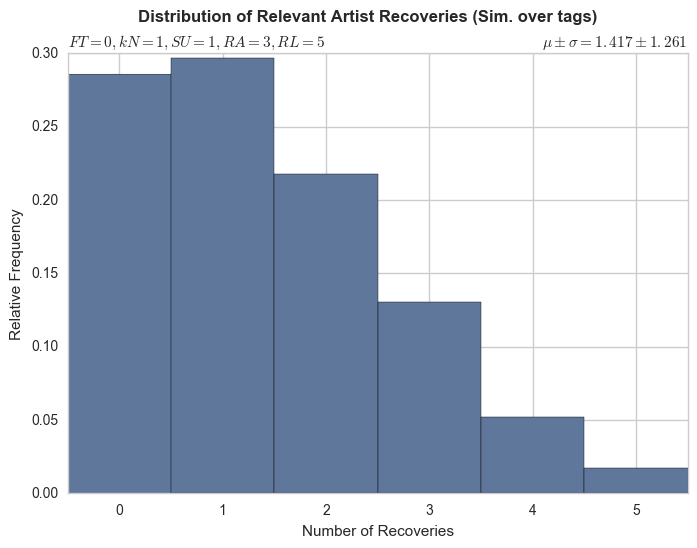
\includegraphics[height=2.4in]{tags,FT=0,kN=1,SU=1,RA=3,RL=5.png}
  \end{subfigure}
  \begin{subfigure}
      \centering
    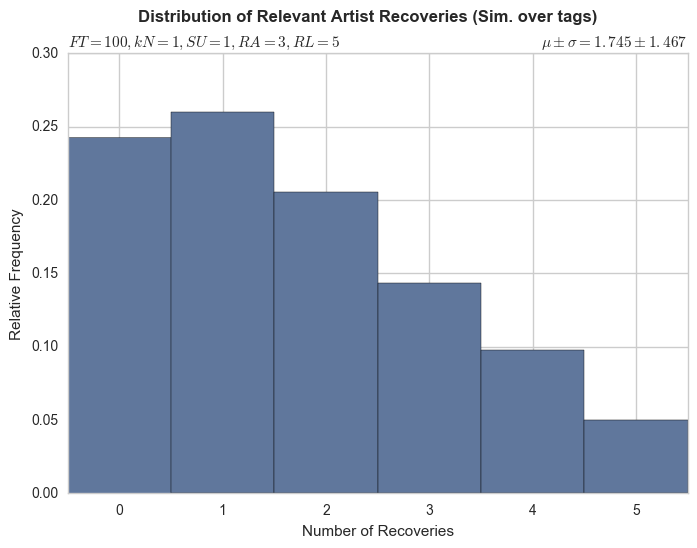
\includegraphics[height=2.4in]{tags,FT=100,kN=1,SU=1,RA=3,RL=5.png}
  \end{subfigure}
  \begin{subfigure}
      \centering
    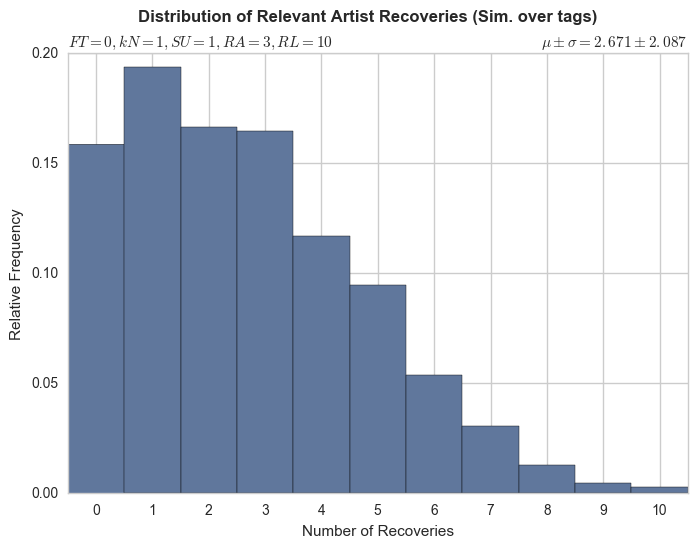
\includegraphics[height=2.4in]{tags,FT=0,kN=1,SU=1,RA=3,RL=10.png}
  \end{subfigure}
  \begin{subfigure}
      \centering
    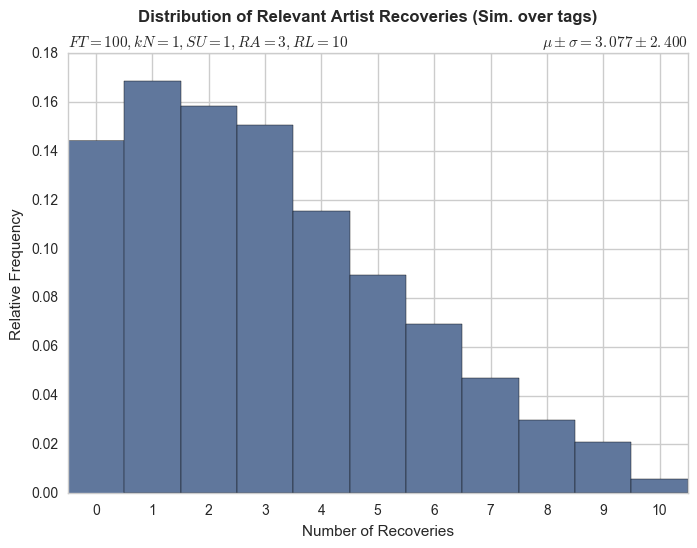
\includegraphics[height=2.4in]{tags,FT=100,kN=1,SU=1,RA=3,RL=10.png}
  \end{subfigure}
  \begin{subfigure}
      \centering
    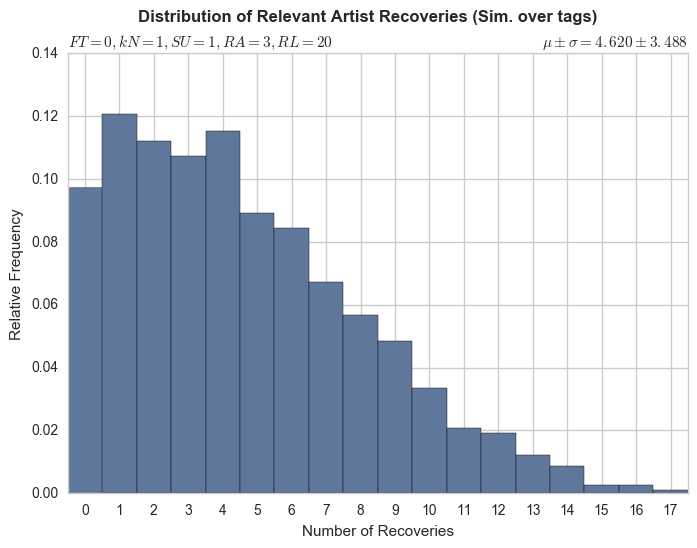
\includegraphics[height=2.4in]{tags,FT=0,kN=1,SU=1,RA=3,RL=20.png}
  \end{subfigure}
  \begin{subfigure}
      \centering
    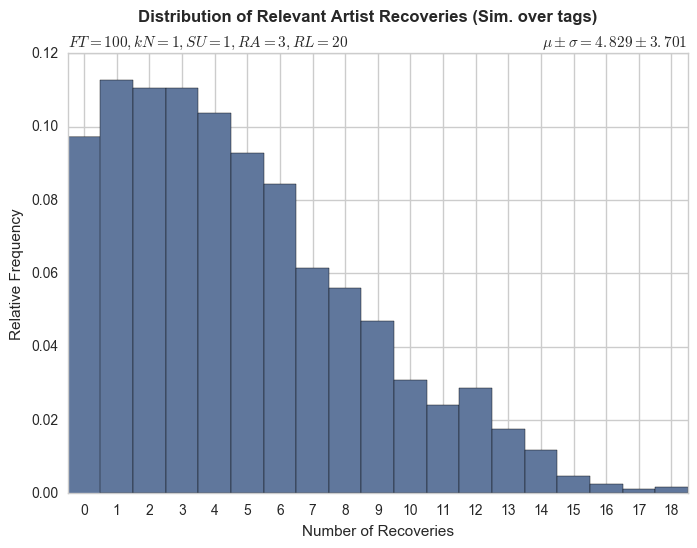
\includegraphics[height=2.4in]{tags,FT=100,kN=1,SU=1,RA=3,RL=20.png}
  \end{subfigure}
\end{figure}

\end{document}